\documentclass[conference]{IEEEtran}
\IEEEoverridecommandlockouts
% The preceding line is only needed to identify funding in the first footnote. If that is unneeded, please comment it out.
%Template version as of 6/27/2024

\usepackage{cite}
\usepackage{amsmath,amssymb,amsfonts}
%\usepackage{algorithmic}
\usepackage{graphicx}
\usepackage{textcomp}
\usepackage{algorithm}
\usepackage{algpseudocode}
\usepackage{xcolor}
\usepackage{amsthm}
\usepackage{my_symbol}
\usepackage{hyperref}
\usepackage{comment}

\newtheorem{theorem}{Theorem}[section] % Theorem environment
\newtheorem{lemma}[theorem]{Lemma} % Lemma environment
\newtheorem{proposition}[theorem]{Proposition} % Proposition environment
\newtheorem{corollary}[theorem]{Corollary}
\theoremstyle{definition}
\newtheorem{definition}[theorem]{Definition} % Definition environment
\newtheorem{example}[theorem]{Example} % Example environment
\newtheorem{remark}[theorem]{Remark} % Remark environment

\begin{document}

\title{Graph Sampling for Scalable and Expressive Graph Neural Networks on Homophilic Graphs}
{
\author{
    \IEEEauthorblockN{Haolin Li, Haoyu Wang, Luana Ruiz}
    \IEEEauthorblockA{Department of Applied Mathematics and Statistics, Johns Hopkins University
    \\\{hli230, hwang320, lrubini1\}@jh.edu}
}
}

\maketitle

\begin{abstract}
Graph Neural Networks (GNNs) excel in many graph machine learning tasks but face challenges when scaling to large networks. GNN transferability allows training on smaller graphs and applying the model to larger ones, but existing methods often rely on random subsampling, leading to disconnected subgraphs and reduced model expressivity. We propose a novel graph sampling algorithm that leverages feature homophily to preserve graph structure. By minimizing the trace of the data correlation matrix, our method better preserves the graph Laplacian trace---a proxy for the graph connectivity---than random sampling, while achieving lower complexity than spectral methods. Experiments on citation networks show improved performance in preserving Laplacian trace and GNN transferability compared to random sampling.
\end{abstract}

\begin{IEEEkeywords}
graph signal processing, graph sampling, graph neural networks, transferability, homophily.
\end{IEEEkeywords}

\section{Introduction}
\label{sec:intro}

GNNs are deep neural networks tailored to network data which have shown great empirical performance in several graph machine learning tasks \cite{gori2005new,kipf17-classifgcnn,defferrard17-cnngraphs,gama18-gnnarchit}. This is especially true in graph signal processing problems---such as recommender systems on product similarity networks \cite{ruiz2020gnns}, or attribution of research papers to scientific domains \cite{hamilton2017inductive}---in which GNNs' invariance and stability properties \cite{ruiz19-inv,gama19-stability} play a key role. 

Yet, in practice most successful applications of GNNs are limited to graphs of moderate size. The sheer size of many modern networks, typically in the order of several millions, frequently makes these models impractical to train. Good results have been seen by leveraging the GNN's transferability property \cite{ruiz20-transf,levie2019transferability}, which states that a GNN with fixed weights produces similar outputs on large enough graphs belonging to the same ``family'', e.g., the same random graph model. This property allows training the GNN on a graph of moderate size, and transferring it for inference on the large graph.

The transferability of GNNs is closely related to their convolutional parametrization, and is a consequence of graph convolutions converging on sequences of graphs that converge to a common graph limit \cite{ruiz2020graphonsp}. Under certain assumptions on the type of limit, and on how the graphs converge to (or are sampled from) them, it is possible to obtain non-asymptotic error bounds inversely proportional to the sizes of the graphs. Such bounds are then used to inform practical considerations, such as the minimum graph size on which to train a GNN to meet a maximum transference error. Once this is determined, the training graph is obtained by sampling a subgraph of the appropriate size at random from the large graph.

Learning GNNs on randomly subsampled graphs works reasonably well on average but, for models trained on small samples, there is large variance in performance, and the worst-case performance can be quite low; see Figure \ref{fig:GNN Acc}. While this is a natural consequence of subsampling any type of data, on graphs issues are exacerbated by the fact that random subgraphs often have disconnected components and isolated nodes. This leads to rank reduction in graph matrix representations, which in turn affects the expressive power of GNNs \cite{ruiz2024spectral}. Indeed, the loss of rank is explicit for the graph Laplacian, in which the multiplicity of the zero eigenvalue indicates the number of connected components in the graph.

Sampling algorithms better at preserving matrix rank---such as spectral algorithms, e.g. \cite{chen2015discrete,anis2016efficient}---or connectivity---such as local algorithms, e.g., breadth-first search\cite{alimohammadi2023localgraphlimitsperspective}---exist, however, spectral methods have high computational complexity, and local methods focus too much on specific regions of the graph and fail to capture global structure.

In this paper, we identify a property that allows graphs to be sampled efficiently without restricting to local regions: feature homophily. Specifically, let $G=(V,E)$ be a graph with node features $X \in \reals^{|V| \times d}$. This graph is feature-homophilic if, given that $(i,j)$ is an edge in $G$, the normalized features $\hat{X}[i,:]$ and $\hat{X}[j,:]$ are close. Our first contribution is to introduce a novel definition of feature homophily based on the graph Laplacian. Then, we show that, by sampling nodes to minimize the trace of the correlation matrix $XX^T$, it is possible to improve the trace of the graph Laplacian, which provides a measure of connectivity of the subsampled graph. 
%which is directly related to graph rank on homophilic graphs. 

This heuristic is formalized as a graph sampling algorithm in Algorithm 1. Unlike other graph sampling routines, it does not require sequential node operations, and has complexity $O(d|E|)$, which is substantially cheaper than other algorithms for large $|V|$ and moderate $d$. 

We conclude with an experimental study of the proposed algorithm on homophilic citation networks, in which we compare it with random sampling. We observe that, for the same sampling budget, our algorithm preserves trace better than sampling at random, and leads to better transferability performance in a semi-supervised learning task.

\section{Preliminaries}

A graph $G=(V,E)$ consists of two components: a set of vertices or nodes $V$, and a set of edges $E \subseteq V \times V$. Generally, graphs can be categorized as being either directed or undirected based on their edge set $E$. A graph is undirected if and only if for any two nodes $u,v \in V$, $(u,v) \in E$ also implies $(v,u) \in E$ (and both correspond to the same undirected edge). In this paper, we restrict attention to undirected graphs.

Let $|V|=n$ be the number of nodes and $|E|=m$ be the number of edges in $G$. Let $\mathbf{A} \in \reals^{n \times n}$ be the corresponding adjacency matrix.
The graph Laplacian is defined as $\mathbf{L} = \mathbf{D} - \mathbf{A}$, where $\bbD=\mbox{diag}(\bbA\boldsymbol{1}_n)$ is the so-called degree matrix. From their definitions, and since $G$ is undirected, we can easily infer that $\mathbf{A}$ and $\bbL$ are symmetric.

In practice, real-world graphs are associated with node data $x \in \reals^n$ called graph signals, where $x[i]$ corresponds to the value of the signal at node $i$. More generally, graph signals consist of multiple features, in which case they are represented as matrices $X \in \mathbb{R}^{n \times d}$ with $d$ denoting the number of features. 

The graph Laplacian plays an important role in graph signal processing (GSP) \cite{shuman13-mag,sandryhaila13-dspg}, as it allows defining the notion of total variation of a signal $x$. Explicitly, the total variation of $x$ is defined as $TV(x)=x^T\bbL x$ \cite{ortega2018graph}. Let $\bbL=\bbV\bbLam\bbV^T$ be the Laplacian eigendecomposition, where $\bbLam$ is a diagonal matrix with eigenvalues ordered as $\lambda_1 \leq \ldots \leq \lambda_n$ and $\bbV$ is the corresponding eigenvector matrix. For unit-norm signals, it is easy to see that the maximum total variation is $\lambda_n$, the largest Laplacian eigenvalue, and the minimum total variation is $\lambda_1=0$, which corresponds to the all-ones eigenvector. Therefore, the Laplacian eigenvalues can be interpreted as graph frequencies, and the eigenvectors as these frequencies' respective oscillation modes.

% \subsection{Graph Neural Networks}

\subsection{Graph Neural Networks} 

GNNs are deep learning models specifically designed for graph-structured data, where each layer consists of two components: a bank of convolutional filters and a nonlinear activation function. 
A graph convolutional filter is the extension of a standard convolutional filter to graph data. More specifically, it consists of a shift-and-sum operation of a signal $x$ on the graph $G$, which is captured by a matrix $\bbS \in \reals^{n\times n}$ encoding the sparsity pattern of the graph, i.e., $\bbS[i,j] \neq 0$ if and only if $(i,j) \in E$ or $i=j$; typical choices are $\bbS=\bbA$ or $\bbS=\bbL$ \cite{segarra17-linear}. The graph shift operator operates on $x$ as $\bbS x$.

\begin{algorithm}[t]
\begin{algorithmic}
    \Require $G(V, E)$, $|V|=n$; $X \in \reals^{n \times d}$; $\gamma \in [0,1]$
    \vspace{2pt}
    \State Calculate deletion budget: $n_d \gets \lfloor (1 - \gamma) \cdot n \rfloor$
    \State Calculate node scores: $\Vec{s} \gets \text{diag}(XX^T)$
    \State Keep $n-n_d$ nodes with the lowest scores:
    
    $\text{idx} \gets \text{argmax}(\Vec{s}, \;\text{descending}=\text{True})[n_d:n]$
    \State Sample graph:
    
    $\tilde{V} \gets V \cap \text{idx}$
    
    $\tilde{E} \gets \{(u,v): u,v \in \tilde{V}, (u,v) \in E \}$
    
    $\tilde{X} \gets X[\text{idx},:]$
    \vspace{2pt}
    \State \Return $\tilde{G}(\tilde{V}, \tilde{E})$; $\tilde{X}$
\end{algorithmic}
\label{alg:sampling}
\caption{Node Sampling for Feature-Homophilic Graphs}
\end{algorithm}

Given any choice of $\bbS$, the graph convolution is defined as $y = \sum_{k=0}^{K-1} h_k \bbS^k x$, where $h_0, \ldots, h_{K-1}$ are the filter coefficients or taps. More generally, for $X \in \reals^{n \times d}$ and $Y \in \reals^{n\times f}$ we can define the convolutional filterbank \cite{gama18-gnnarchit}
\begin{equation}
     Y = \sum_{k=0}^{K-1} \bbS^k X \bbH_k
\end{equation}
where $\bbH_k \in \reals^{d \times f}$, $0 \leq k \leq K-1$.
%, mapping features from $\reals^d$ to $\reals^f$.

The $\ell$th layer of a GNN is given by \cite{gama18-gnnarchit}
\begin{equation}
    X_{\ell} = \sigma \bigg( \sum_{k=0}^{K-1} \bbS^k X_{\ell-1} \bbH_{\ell k}\bigg)
\end{equation}
with $\sigma: \reals \to \reals$ an entry-wise nonlinearity (e.g., the ReLU or sigmoid). At layer $\ell=1$, $X_0$ is the input data, and the last layer output $X_L$ is the output $Y$ of the GNN. For succinctness, in the following we will represent the whole $L$-layer GNN as a map $Y = \Phi(X,G;\ccalH)$ with $\ccalH=\{\bbH_{\ell k}\}_{\ell,k}$.

\subsection{Transferability of GNNs}

The mathematical property that allows training GNNs on small graph subsamples of larger graphs is their transferability. Explicitly, GNNs are transferable in the sense that when a GNN with fixed weights $\ccalH$ is transferred across two graphs in the same ``family'', the transference error is upper bounded by a term that decreases with the graph size. Typical transferability analyses show this by defining graph ``families'' as graphs coming from the same random graph model, or converging to a common graph limit. Here, we consider families of graphs identified by the same graphon, which can be seen as both a generative model and a limit model for large graphs. 

A graphon is a bounded, symmetric, measurable function $\bbW: [0,1]^2 \to [0,1]$ \cite{borgs2008convergent,lovasz2012large}. Graphs can be sampled from $\bbW$ by sampling nodes $u_1, \ldots, u_n$ from $[0,1]$, and sampling edges $(u_i,u_j)$ with probability $\bbW(u_i,u_j)$. The graph limit interpretation is more nuanced but has to do with the fact that, on sequences of graphs converging to $\bbW$, the densities of certain ``motifs'', e.g., triangles, also converge. For graphs associated with the same graphon, we have the following transferability theorem.

\begin{theorem}[GNN transferability, simplified \cite{ruiz2021transferability}]
    Let $\Phi$ be a GNN with fixed coefficients, and $G_n$, $G_m$ graphs with $n$ and $m$ nodes sampled from a graphon $\mathbf{W}$. Under mild conditions, $\| {\Phi}(G_n) - {\Phi}(G_m) \|= \mathcal{O}(n^{-1} + m^{-1})$ w.h.p.
\end{theorem}

In this paper, we will use the transferability property of GNNs, together with a novel graph sampling algorithm, to train GNNs on small graph subsamples and ensure they scale well to large graphs.

\begin{figure*}[t]
\centering
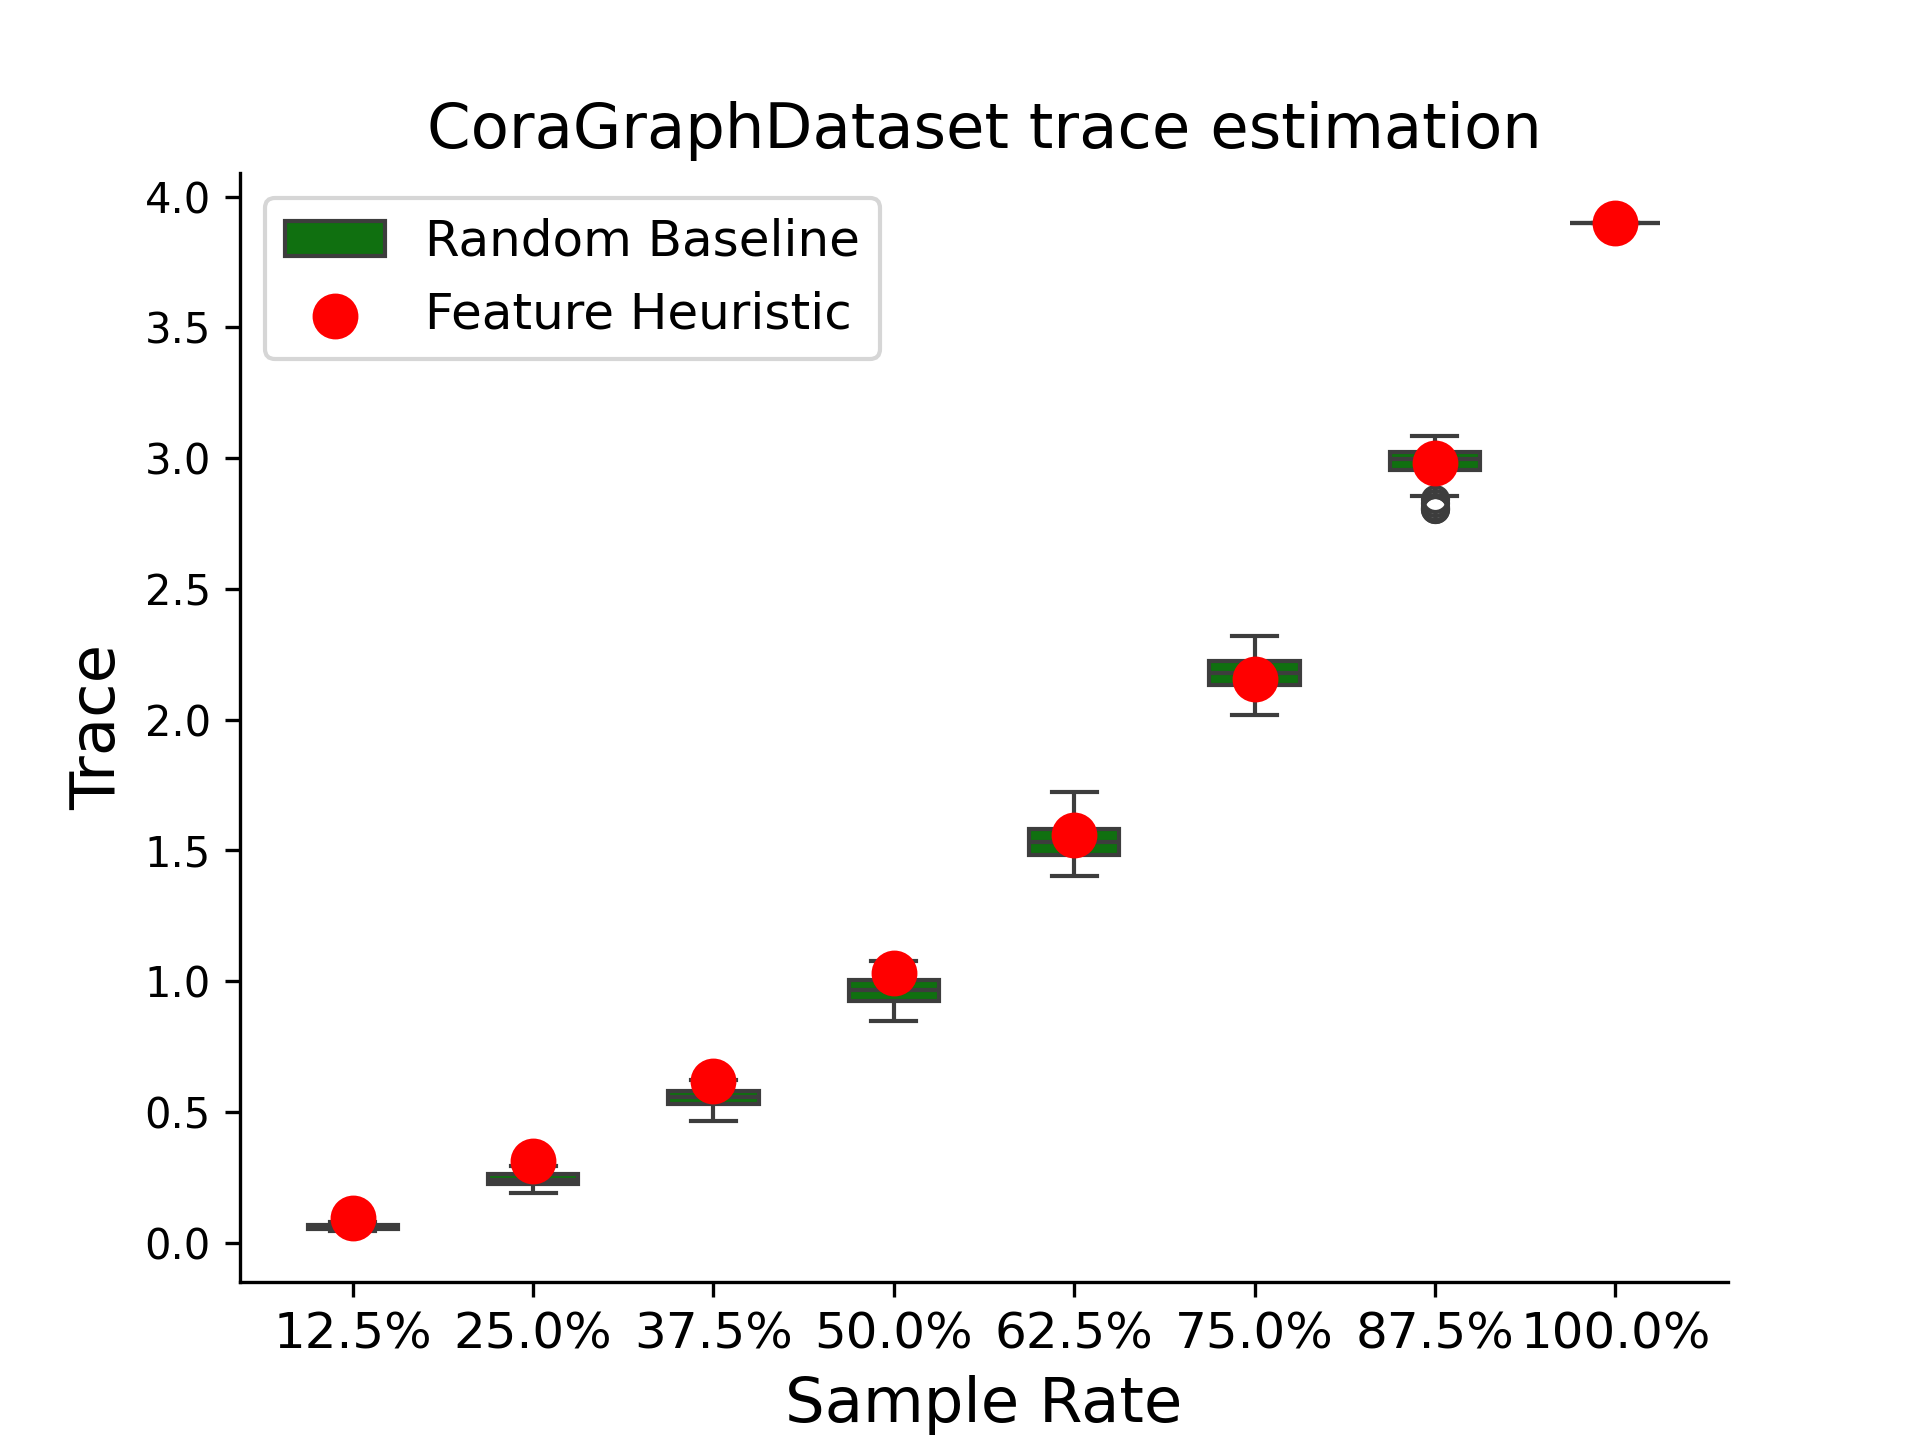
\includegraphics[height=4cm,width=0.32\textwidth]{img/trace_revised/CoraGraphDataset_trace_boxplot.png}
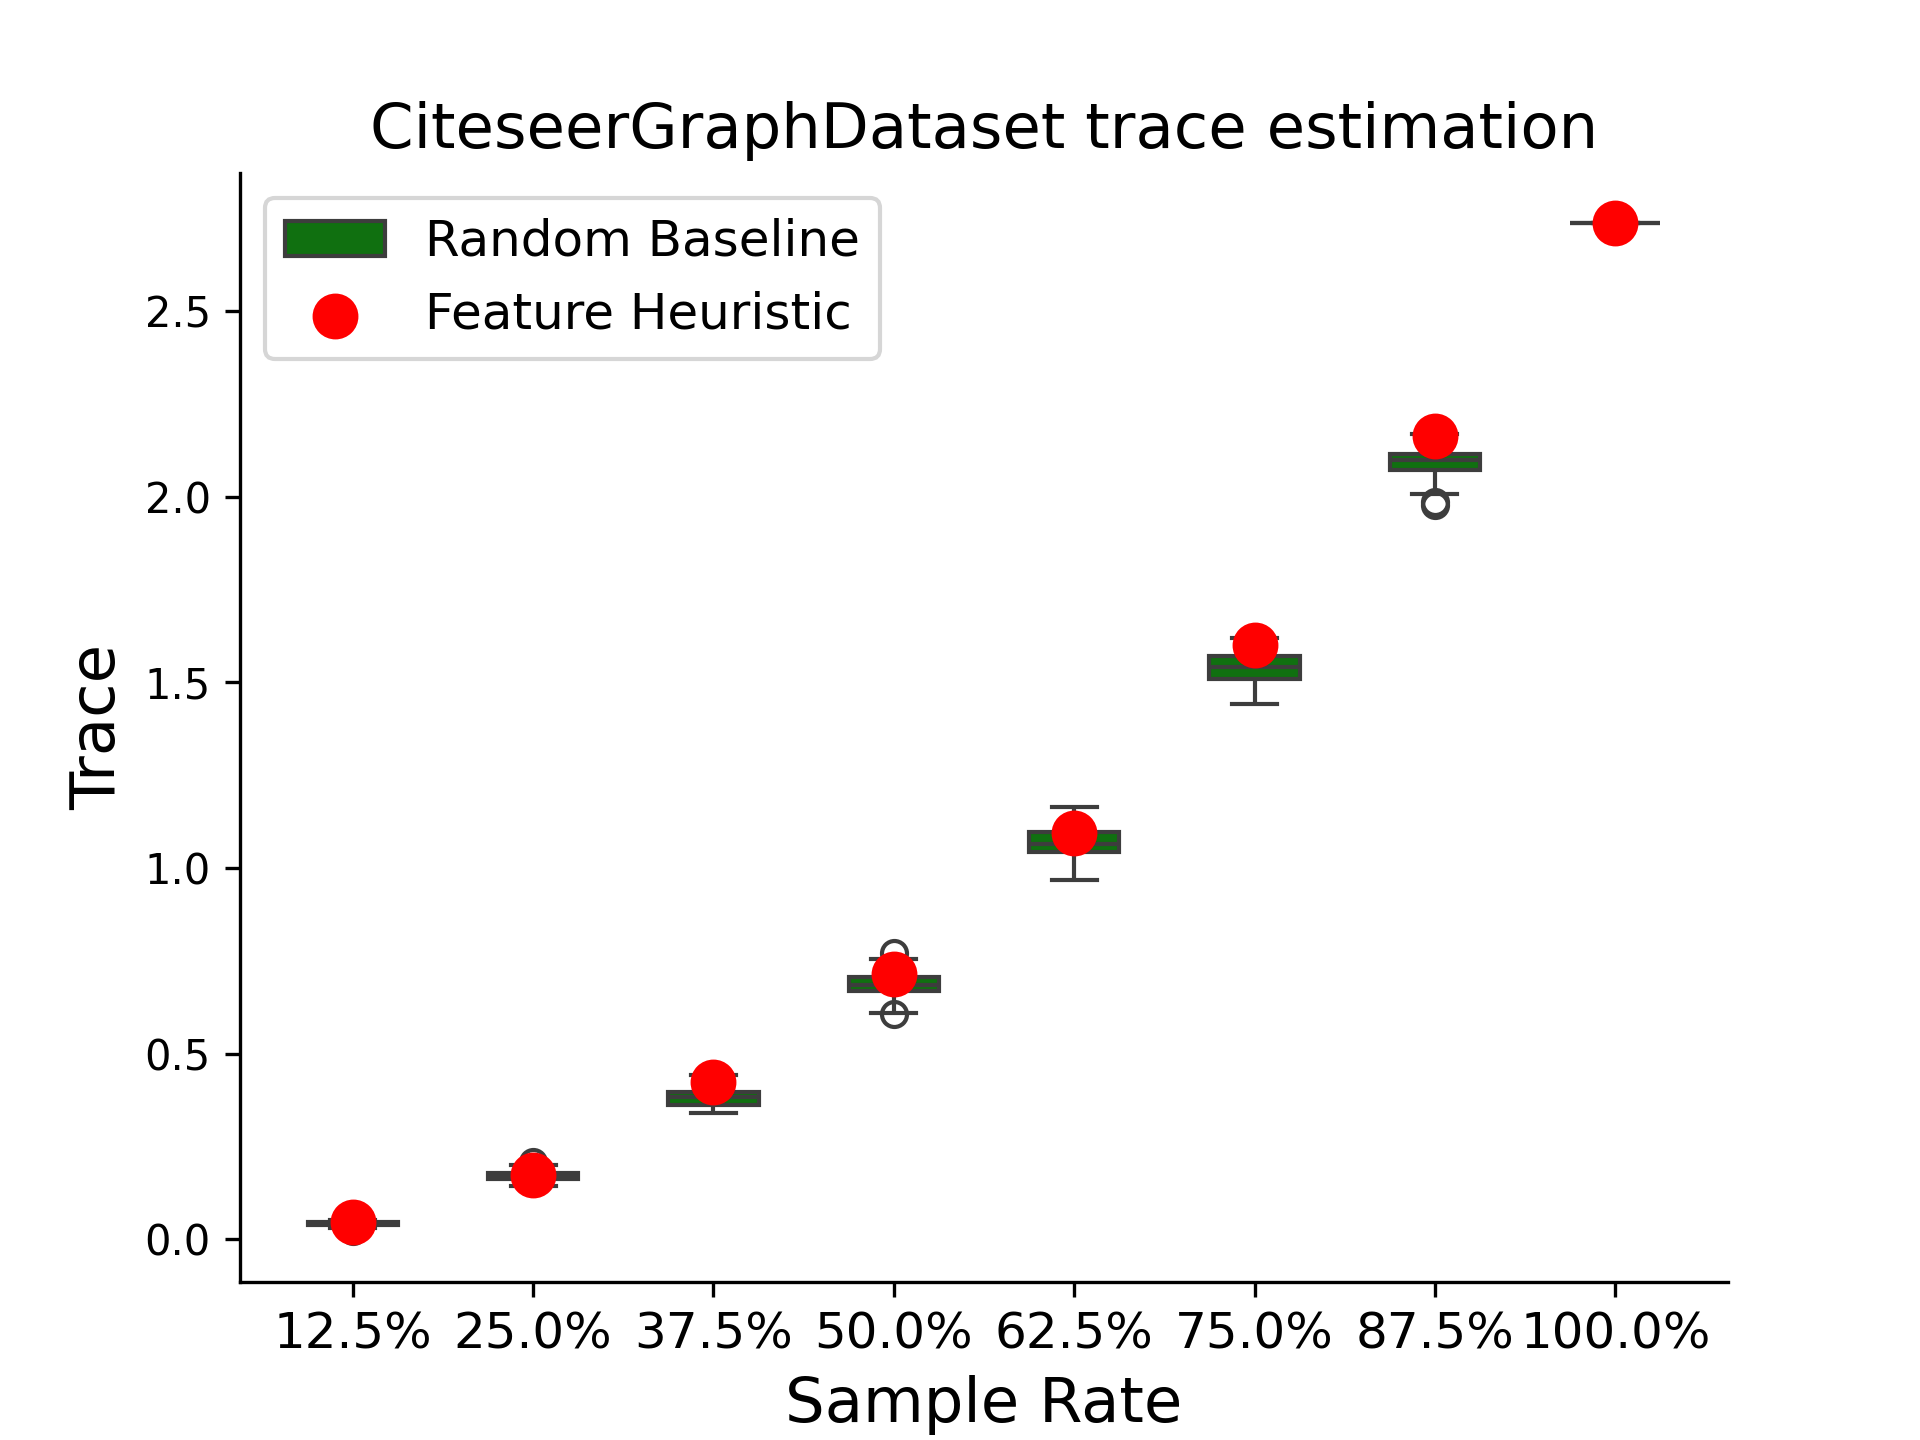
\includegraphics[height=4cm,width=0.32\textwidth]{img/trace_revised/CiteseerGraphDataset_trace_boxplot.png}
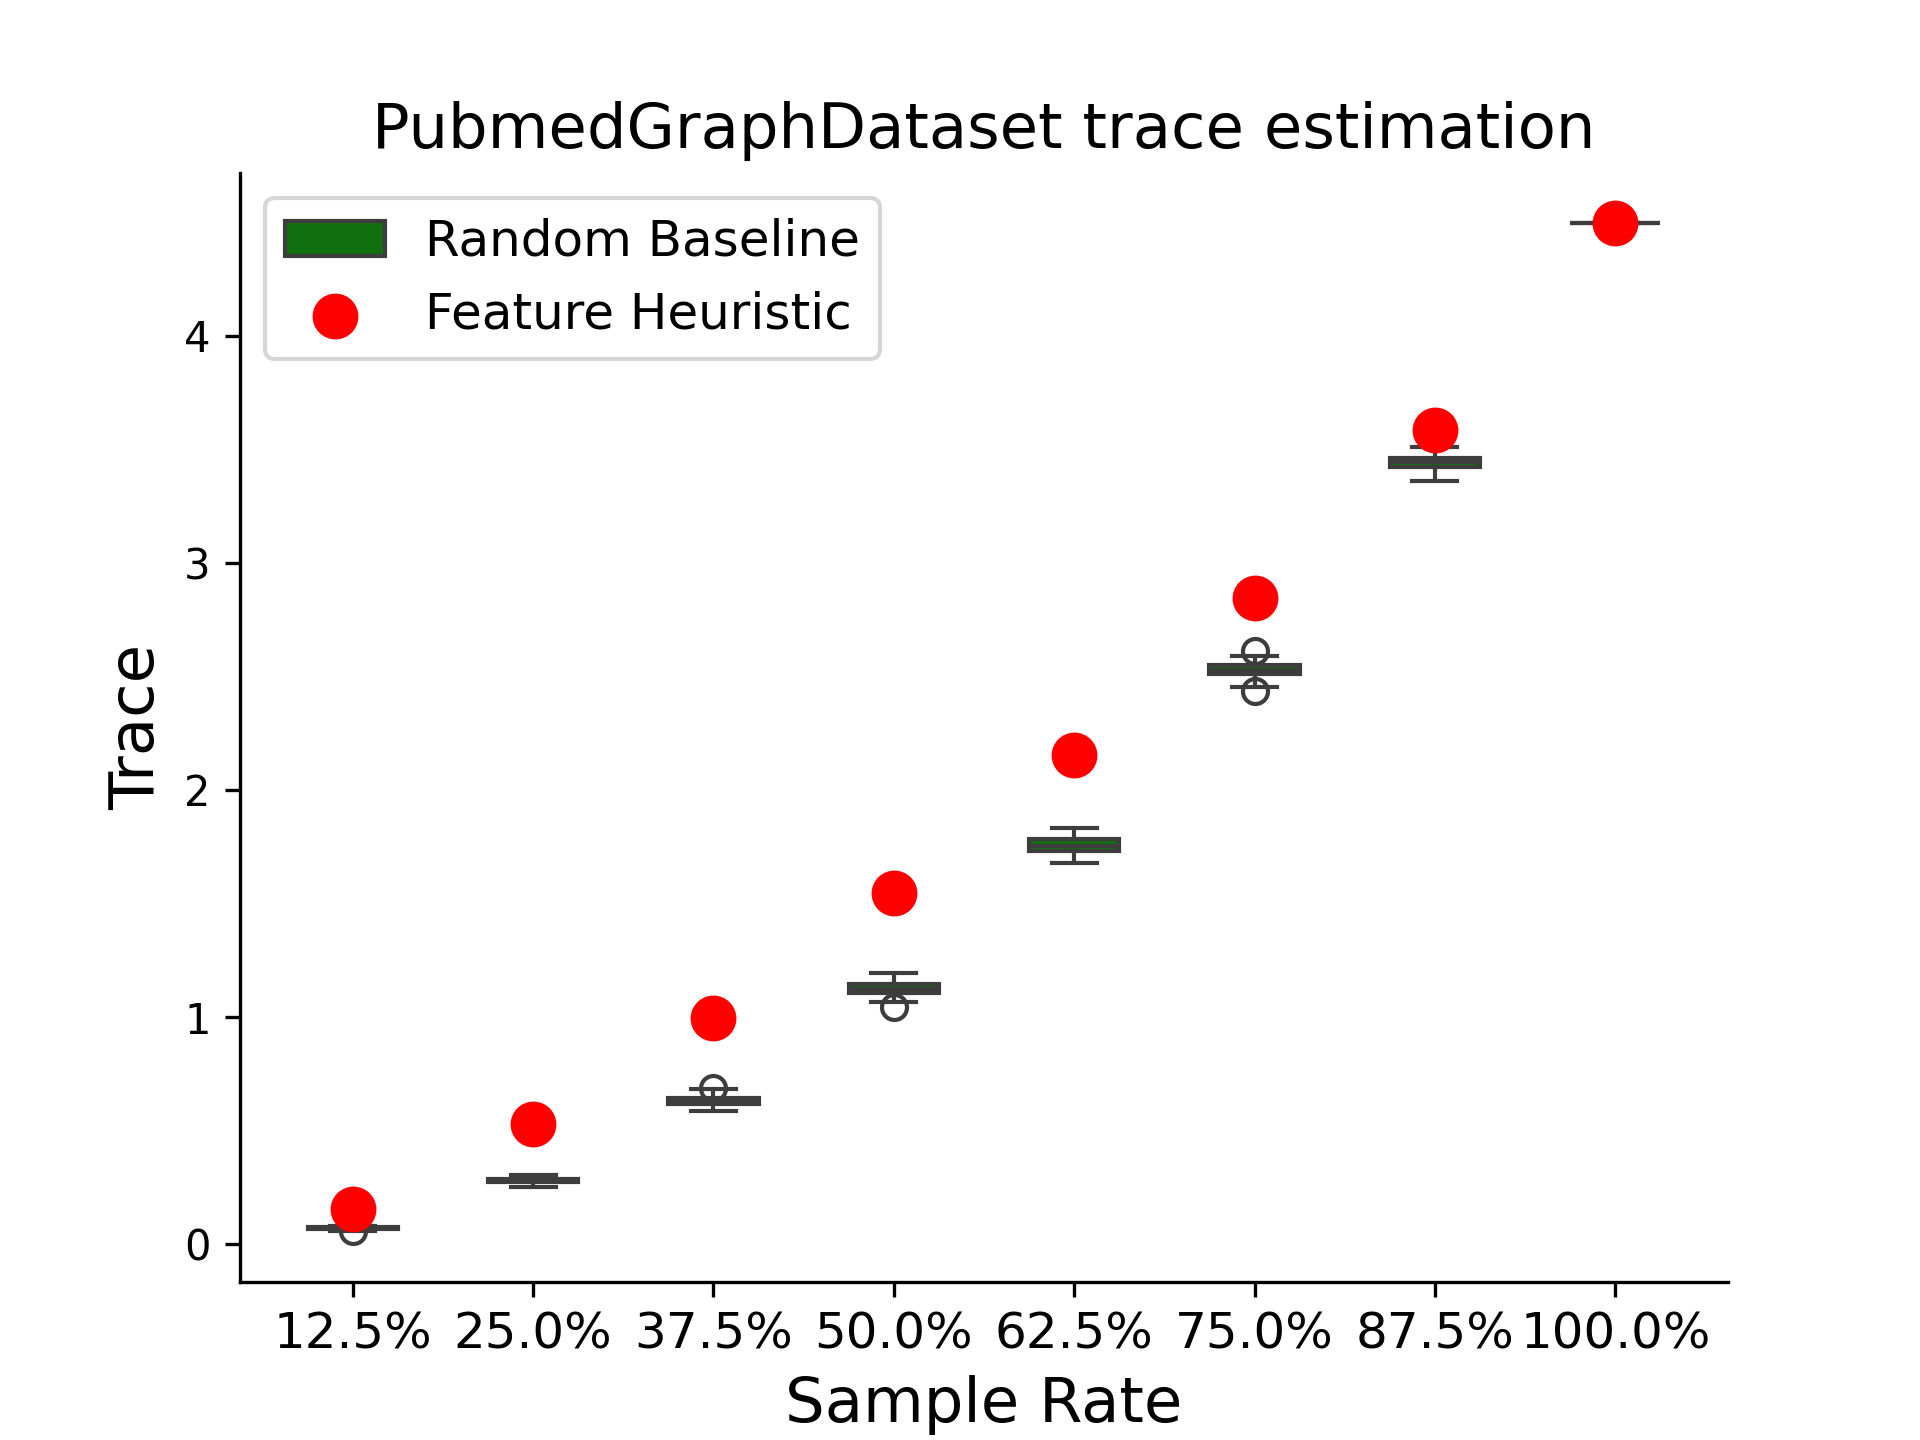
\includegraphics[height=4cm,width=0.32\textwidth]{img/trace_revised/PubmedGraphDataset_trace_boxplot.png}
\caption{Adjusted Laplacian trace versus graph subsampling rate. The adjusted trace is the subsampled graph Laplacian trace normalized by the number of sampled nodes. Boxplots indicate the mean and standard error of the trace obtained from 50 rounds of random node subsampling; red dots are the trace of subgraphs generated using our sampling heuristic (Algorithm 1). Trace preservation is almost always better for our algorithm compared with the average of random subsampling, except for Cora at 75\% sample rate.}
\label{fig:trace}
\end{figure*}

\begin{figure}
    \centering    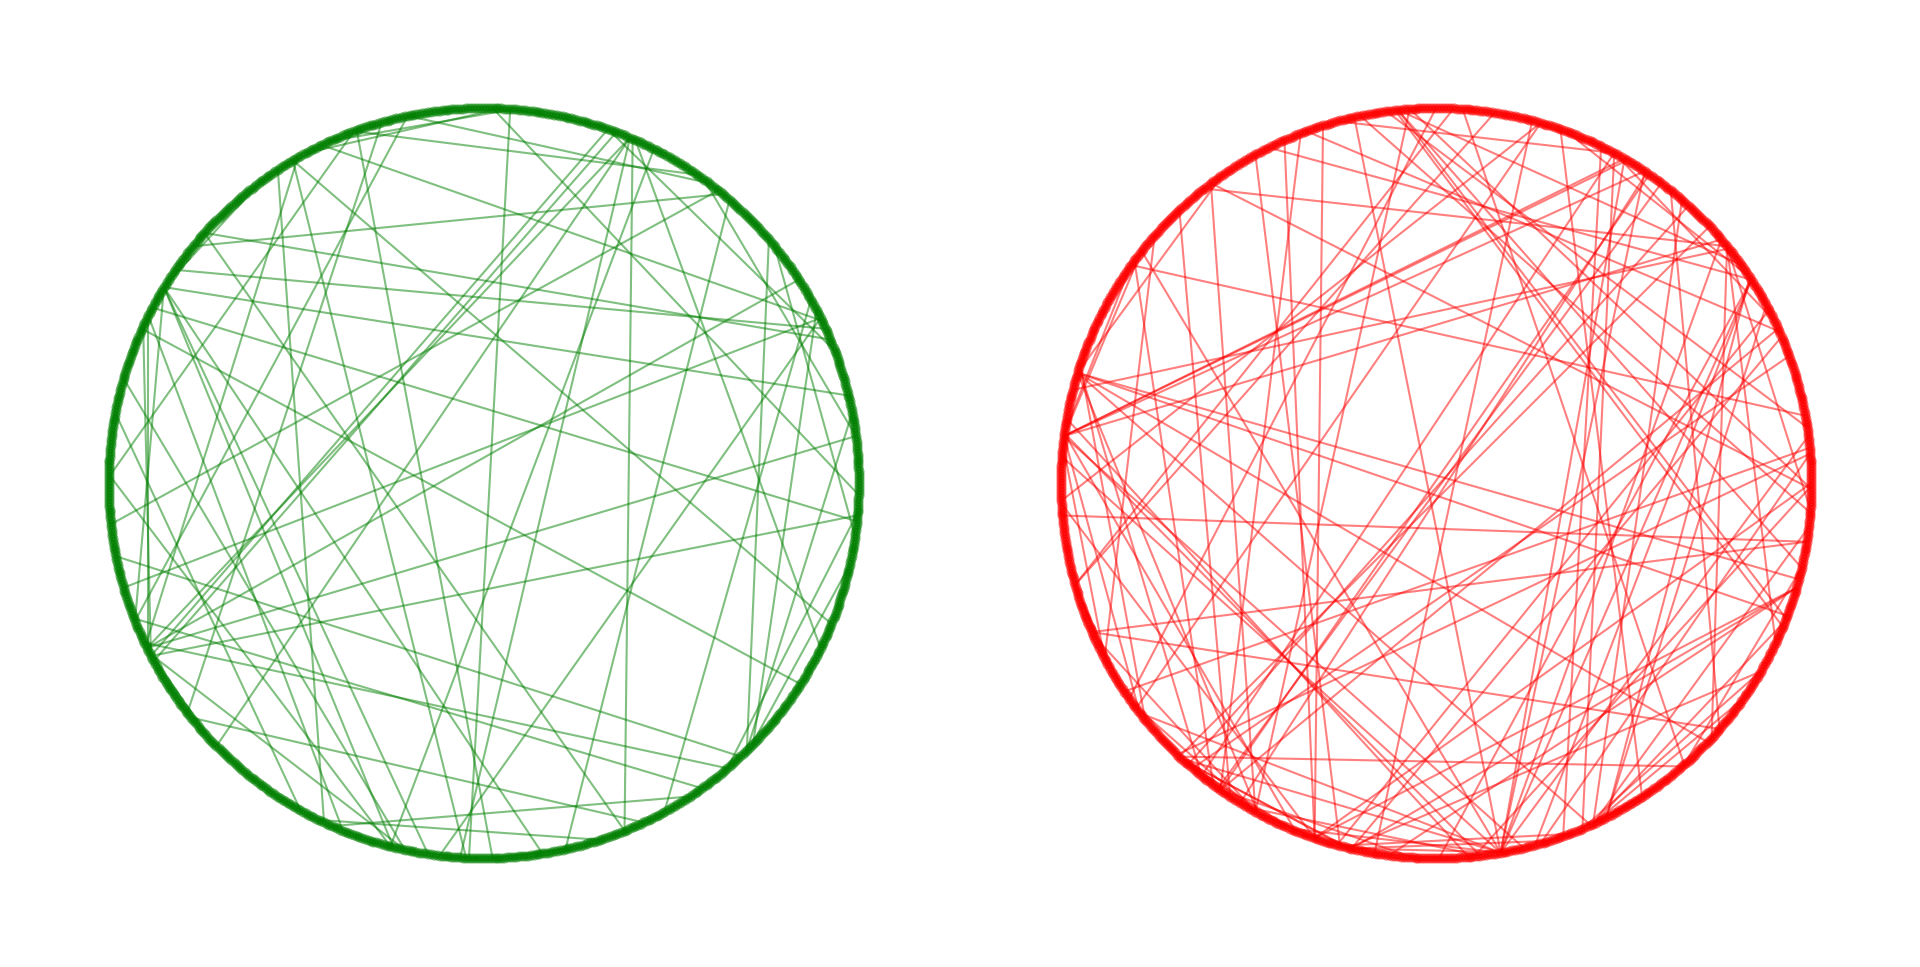
\includegraphics[width=0.95\linewidth]{img/feature_heuristic.png}
    \caption{Example of randomly sampled subgraph (green) and subgraph sampled using Algorithm 1. Both graphs have 800 nodes and were sampled from the PubMed citation network, which has 19,717 nodes.}
    \label{fig:pubmed_example}
\end{figure}

\subsection{Expressive Power of GNNs}

While GNNs achieve remarkable performance in many graph machine learning tasks, they have fundamental limitations associated with their expressive power \cite{xu2018how,chen2019equivalence}. In GSP problems specifically, the expressivity of a GNN is constrained by the expressivity of the graph convolution, which in turn is constrained by the rank of the graph shift operator \cite{ruiz2024spectral}. This is demonstrated in the following proposition.

\begin{proposition}[Expressivity of Graph Convolution]
Let $G$ be an $n$-node symmetric graph with rank-$r$ graph shift operator $\mathbf{S}$, $r < n$, and $x \in \reals^n$ an arbitrary graph signal. Consider the graph convolution $\hat{y} = \sum_{k=0}^{K-1}h_k\mathbf{S}^kx$. Let $\ccalY \subset \reals^n$ be the subspace of signals that can be expressed as $y=\hat{y}$ for some $h_0, \ldots, h_{K-1}$. Then, $dim(\ccalY) \leq r + 1$.
\end{proposition}
\begin{proof}
   See the extended version, available \href{https://github.com/JamesLi128/Graph-Sampling-for-Scalable-and-Expressive-Graph-Neural-Networks-on-Homophilic-Graphs/blob/master/main.pdf}{here}. 
\end{proof}

In other words, the space of signals that can be represented with a graph convolution shrinks with the rank of the graph shift. Rank preservation is thus an important consideration when sampling subgraphs for GNN training. We will focus on the more tractable problem of preserving the Laplacian trace, which can be seen as a continuous proxy of its rank. 

\begin{figure*}[t]
\centering
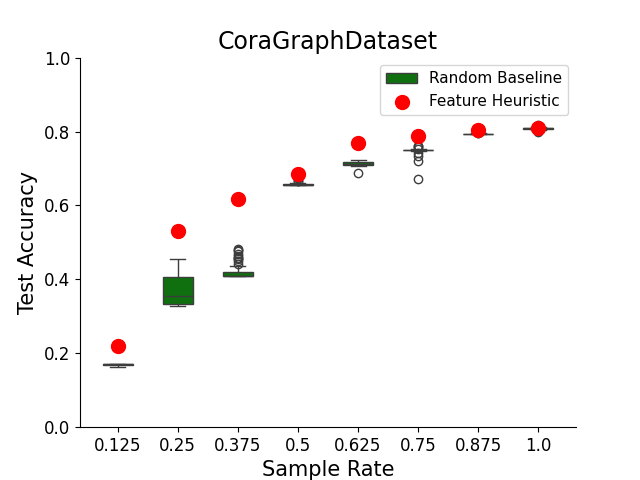
\includegraphics[height=4cm,width=0.32\textwidth]{img/GNN_acc_revised/CoraGraphDataset_undirected_random_baseline_boxplot.png}
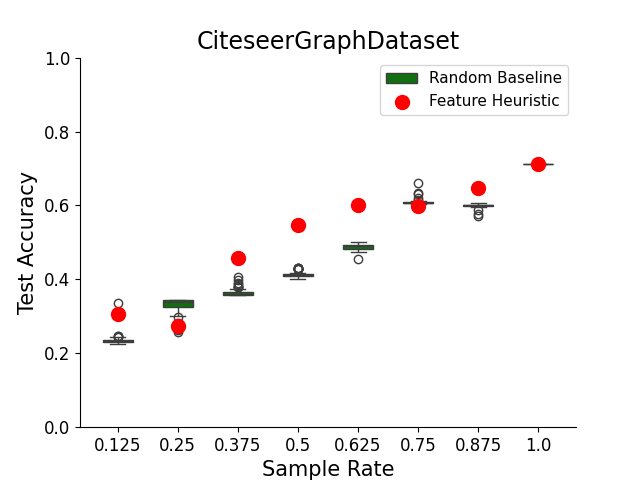
\includegraphics[height=4cm,width=0.32\textwidth]{img/GNN_acc_revised/CiteseerGraphDataset_undirected_random_baseline_boxplot.png}
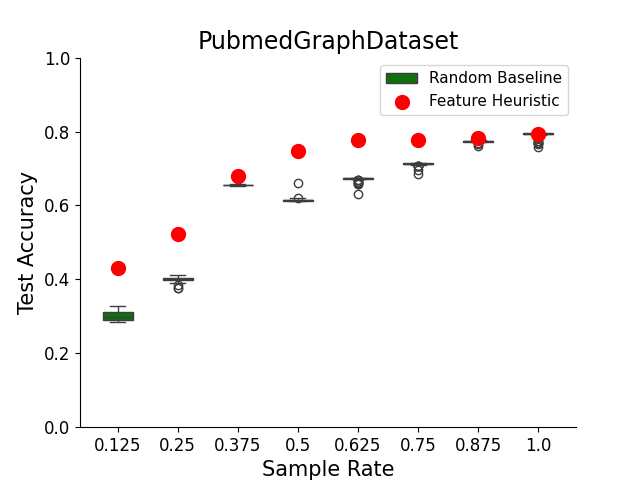
\includegraphics[height=4cm,width=0.32\textwidth]{img/GNN_acc_revised/PubmedGraphDataset_undirected_random_baseline_boxplot.png}
\caption{Test accuracy achieved by GNN on full graph versus training graph subsampling rate. Boxplots indicate the spread of the accuracy realized by GNNs trained on 50 random node-induced subgraphs; red dots are the test accuracy of GNNs trained on subgraphs produced by our heuristic (Algorithm 1). The feature-based heuristic yields better results across the board, except for CiteSeer at 25\% sample rate.}
\label{fig:GNN Acc}
\end{figure*}

\section{Feature homophily and homophily-based sampling}

We start by introducing the notion of feature homophily.
%, which is a requirement for our algorithm.
In order to make this definition compatible for graphs of different sizes and with different features features, we first need to normalize $X \in \mathbb{R}^{n\times d}$ along both the feature and node dimensions. Explicitly, let $\Vec{\mu} = (\mu_1, \cdots, \mu_d)^T \in \mathbb{R}^d$ be the mean feature vector and $\Vec{\sigma} = (\frac{1}{\sigma_1}, \cdots, \frac{1}{\sigma_d})^T \in \mathbb{R}^d$ the standard deviation vector. We define the normalized graph feature matrix as:
\begin{equation} \label{eqn:norm_features}
    \hat{X} = (X - \mathbf{1}_n \Vec{\mu}^T) \odot (\frac{1}{\sqrt{d}} \cdot \mathbf{1}_n \Vec{\sigma}^T) \text{.}
\end{equation}
I.e., $\hat{X}[i,j] = \frac{X[i,j] - \mu_j}{\sqrt{d}\sigma_j}$. 

\begin{definition}[Feature Homophily] \label{def:feature_homophily}
    Let $G$ be a graph with Laplacian matrix $\bbL$, and let $\hat{X}$ be the corresponding normalized feature matrix \eqref{eqn:norm_features}. The feature homophily of graph $G$ is defined as:
    \begin{equation} \label{eqn:feature_homophily}
        h_G = \frac{1}{n} \cdot {tr}(-\mathbf{L}\hat{X}\hat{X}^T)\text{.}
    \end{equation}
\end{definition}

Since $\bbL$ is positive semidefinite and the trace of the outer product is the product of traces, it is ready to see, by Cauchy-Schwarz, that $h_G \leq 0$ for any undirected graph $G$. The larger the feature homophily $h_G$, i.e., the closer it is to $0$, the higher the alignment of the data $X$ (or, more precisely, of its principal components) with the low-frequency eigenvectors of $\bbL$---which account for most of the graph's global structure such as its connected components and clusters/communities. Thus, the data is informative with regards to the graph. On the other hand, highly negative values of $h_G$ indicate strong alignment of $\hat{X}$ with high-frequency eigenvectors, which tend to be noisier and less descriptive of the graph structure.

The following proposition provides a lower bound on ${tr}(\bbL)$ in terms of the feature homophily $h_G$.
\begin{proposition}[Lower Bound on ${tr}(\bbL)$]
    \label{bound on tr L}
    \begin{equation} \label{eqn:bound_tr_L}
        \text{tr}(\bbL) \geq - \frac{nh_G}{\text{tr}(\hat{X}\hat{X}^T)}
    \end{equation}
\end{proposition}
%\textcolor{orange}{J:It looks wired if I put the proof of proposition 3.3 inside the proof of 3.2 because there's no clear division between the statement and the proof of 3.3.w}
\begin{proof}
See the extended version, available \href{https://github.com/JamesLi128/Graph-Sampling-for-Scalable-and-Expressive-Graph-Neural-Networks-on-Homophilic-Graphs/blob/master/main.pdf}{here}.
\end{proof}

Note that if the graph $G$ has high feature homophily, the right-hand side of \eqref{eqn:bound_tr_L} is small and the lower bound on $tr(\bbL)$ is approximately vacuous. For heterophilic graphs, $h_G$ has higher magnitude, so the lower bound is further away from zero.

\subsection{Sampling Heuristic for Homophilic Graphs}

Although simple, the result in Proposition \ref{bound on tr L} has important implications for feature-homophilic graph sampling. Assume we start removing nodes from $G$ according to the diagonal entries of $X X^T$ sorted in decreasing order, so that the denominator on the right-hand side of \eqref{eqn:bound_tr_L} becomes progressively smaller. We prioritize removing nodes corresponding to the largest diagonal elements because, in order to tighten the lower bound of ${tr}(\bbL)$, we should enforce the denominator ${tr}(\hat{X}\hat{X}^T)^2$ to be as small as possible, given that the graph is homophilic. Hence, deleting from largest to smallest makes sense. This idea is formalized in Algorithm 1.

When $d<n$, as is often the case in practice, Algorithm 1 offers lower computational complexity than graph sampling algorithms which mazimize the graph Laplacian trace directly, as demonstrated by Proposition \ref{prop:complexity}.

\begin{proposition}[Complexity of Algorithm 1] \label{prop:complexity}
    Let $G=(V,E)$ be a graph with $|V|=n$ and $|E|=m$, and let $X \in \reals^{n\times d}$ be the corresponding node feature matrix. For any sampling budget $\gamma$, the complexity of Algorithm 1, including computation of $h_G$, is $O(dm)$. If $G$ is known to be feature-homophilic, computation of $h_G$ can be bypassed and the complexity simplifies to $O(dn)$. 
\end{proposition}
\begin{proof}
See the extended version, available {\href{https://github.com/JamesLi128/Graph-Sampling-for-Scalable-and-Expressive-Graph-Neural-Networks-on-Homophilic-Graphs/blob/master/main.pdf}{here}}.
\end{proof}

Importantly, the complexity of Algorithm 1 is dominated by the complexity of calculating the feature homophily, which only has to happen once prior to execution to determine if the graph is homophilic. The complexity is further independent of the sampling budget, as the diagonal elements of $XX^T$ only have to be computed and sorted once. 

On sparse graphs ($m \ll n^2$) with moderate feature dimension $d$, Algorithm 1 is cheaper than direct maximization of $tr(\bbL)$, which requires $O((1-\gamma)n^2)$ computations---$O(n)$ node degree computations $(1-\gamma)n$ times, as node degrees change each time a node is removed from $G$. In fact, this is an underestimation, as it does not factor in the cost of breaking ties across nodes with the same degree. Algorithm 1 is also notably cheaper than spectral algorithms such as \cite{chen2015discrete,anis2016efficient} which are inspired by E-optimal sampling and, without exhaustive search, require greedy routines with complexity at least $O(\gamma nm)$. Another advantage of Algorithm 1 is that it does not require sequential execution, unlike maximization of $tr(\bbL)$ and \cite{chen2015discrete,anis2016efficient}, which cannot be parallelized.

\subsection{Connections with Orthogonality,  Leverage Scores Sampling, and Further Discussion}

Our feature homophily definition provides insights into {graph alignment and orthogonality}. More specifically, $h_G$ can be interpreted as an {inner product} between the Laplacian $\mathbf{L}$ and the feature correlation matrix $\hat{X} \hat{X}^T$. High homophily (i.e., $h_G \approx 0$) implies that the graph Laplacian and the feature correlation matrix are almost orthogonal.

The feature homophily score can also be rewritten as a weighted $\ell_1$-norm of the adjacency matrix, where the weight of each edge $A_{ij}$ is the squared Euclidean distance between feature vectors $X_i$ and $X_j$~\cite{kalofolias2016learn}. This formulation connects homophily with {graph sparsity}, suggesting that our sampling heuristic could serve as a {structured sparsification technique} for large-scale graphs similar to graph sparsification techniques based on effective resistances \cite{spielman2011graph}.

The sampling method we propose in Algorithm 1 has interesting connections with {leverage scores sampling} approaches used in regression models. In classical settings, leverage scores quantify the influence of data points on the regression outcome. However, unlike traditional leverage score sampling, which retains influential, high-leverage points, our approach removes the nodes with the largest scores.

To formalize this connection, recall that leverage scores sampling is based on the diagonals of the hat matrix $\mathbf{H} = X (X^T X)^{+} X^T$.
Since $\mathbf{H}$ is positive semidefinite, its diagonal is always nonnegative. Using the singular value decomposition (SVD) of $X$, $X = U \Sigma V^T$,
we can decompose the hat matrix as $\mathbf{H} = U \Sigma V^T (V \Sigma^2 V^T)^{+} V \Sigma U^T = U_r U_r^T$, thus the images of both $X$ and $\mathbf{H}$ lie in the span of $U$. Examining the diagonal of $XX^T = U\Sigma^2U^T$, we observe that the node scores computed in our algorithm are {effectively leverage scores weighted by the singular values of} $X$. 
Our approach removes nodes that contribute disproportionately to the feature covariance structure, regularizing the selection.

This criterion aligns with the goal of {preserving Laplacian rank}: since the multiplicity of the zero eigenvalue counts the number of connected components, removing nodes that form separate components or have low connectivity minimally affects the overall structure. Specifically, if a graph initially has $n$ nodes and $k$ connected components (so that $\text{rank}(\mathbf{L}) = n - k$), removing an isolated node decreases both $n$ and $k$ by one, preserving the rank at $n - k$. This suggests that our method implicitly filters out nodes that contribute little to the global structure while retaining the essential connectivity properties of the original graph.

\begin{comment}
\red{Add something on graph orthogonality.}

\red{On the other hand, our method is also relevant to the idea of leverage score sampling used in regression models. In fact, the node scores $\Vec{s}$ computed in the algorithm fit into the definition of leverage scores by David Woodruff\textbf{[REFERENCE CHECK NEEDED]}. However, the key difference is, in regression models we tend to keep data points with high leverage scores due to their greater influence on the result of the regression, but in our approach we instead remove the rows with the largest scores.

To see the connection between our work and traditional leverage score sampling, we make the following analysis. The leverage score sampling considers the diagonals of the hat matrix $\mathbf{H} = X (X^T X)^{+} X^T$. Notice that the diagonals are always nonnegative because $\mathbf{H}$ is positive semidefinite. First, we consider the SVD decomposition of the feature matrix X 
\[
X = U \Sigma V^T
\]
where $U = \begin{bmatrix} U_r & U_\perp \end{bmatrix}, 
\Sigma = \begin{bmatrix} \Sigma_r & 0 \\ 0 & 0 \end{bmatrix},
V = \begin{bmatrix} V_r & V_\perp \end{bmatrix}$. Then the hat matrix can be decomposed as follows:

\[
\textbf{H} = U \Sigma V^T (V \Sigma^2 V^T)^{+} V \Sigma U^T.
\]

\[
\textbf{H} = U_r U_r^T.
\]

The first observation is that both the image of X and $\mathbf{H}$ are the subspaces of the linear span of $U$. A more insightful examination on the diagonals of $XX^T$ as follows shows that the node scores $\Vec{s}$ calculated in our algorithm are essentially the leverage scores weighted by the singular values of $X$.

\[
XX^T = U \Sigma V^TV\Sigma U^T = U\Sigma^2U^T
\]

It is a well known fact that the multiplicity of zero eigenvalues of a graph's Laplacian equals the number of connected components in the graph. Consequently, if we want to select a subgraph while preserving the Laplacian's rank as much as possible, it is optimal to delete isolated or separately connected nodes. Concretely, suppose the original graph has n nodes and k connected components, so its Laplacian has rank $n - k$. If we remove one node that forms its own component(reducing both n and k by one), the new graph's Laplacian still has rank $(n-1) - (n-k) = n-k$, thus preserving the original Laplacian's rank.}

\end{comment}

\section{Experimental Results}

In this section, we present an empirical analysis of our sampling algorithm on citation networks. Specifically, we compare the test accuracy achieved by GNN models trained on subgraphs sampled using our heuristic and the random node sampling baseline on the full size graph. 

\noindent \textbf{Trace preservation.} %Among many ways to evaluate a sampling algorithm over a graph, apart from test accuracy benchmarks which we will show in Figure \ref{fig:GNN Acc}, an informative one is the rank of $\mathbf{L}$. However, because the estimation on the rank of $\mathbf{L}$ is almost infeasible due to the high dimensionality, trace is often used as an intermediate.
First, we investigate the ability of our heuristic to preserve Laplacian trace in three homophilic citation networks. In agreement with the lower bound derived in Proposition \ref{bound on tr L}, in Figure \ref{fig:trace} we see that across all datasets, our sampling method results in subgraphs with larger adjusted $\tilde{{tr}}(\textbf{L}) = {tr}(\mathbf{L}) / n$. This pattern is especially visible for PubMed, as exemplified by the 800-node subsamples in Figure \ref{fig:pubmed_example}. Clearly, the graph sampled using Algorithm 1 is more connected than its random counterpart.

\noindent \textbf{GNN training.} Next, we investigate the transferability of GNNs trained on subgraphs sampled using our heuristic and subgraphs and random node-induced subgraphs. Specifically, we train a GNN model on graphs of size given by the $x$-axis of Figure \ref{fig:GNN Acc}, and report their test accuracy on the full size graph. 

\noindent \textbf{Experiment details.} For each dataset and sample rate, we chose hidden dimension in $\{64, 128\}$, number of layers in $\{1,2,3\}$, number of epochs in $\{200, 300\}$, learning rate and weight decay in $\{0.001, 0.0001\}$, GCN model type in $\{\text{GCN}, \text{SAGE}\}$ with ReLU activations, all optimized using Adam \cite{kingma17-adam}. All of the graphs are symmetrized beforehand, turning directed edges into undirected ones. 

%It is worth mentioning that the GNN of our choice is rather simple. This is because the power of a sampling method can be more apparent and easier to identify if model complexity is relatively restrained.
In Figure \ref{fig:GNN Acc}, the box plots represent the mean and standard error of the accuracy achieved over 50 rounds, and the red dots the test accuracy achieved by our model.  Our sampling heuristic is substantially better, except for CiteSeer at sample rate 25\%. Notably, at a sample rate of 62.5\%, our heuristic beat random by around 10\% for all three datasets.

%\section{Conclusions}

%In this paper, we introduced a novel graph sampling algorithm that leverages feature homophily to efficiently preserve the structural properties of large graphs. 

%Compared with random sampling, our proposed sampling heuristic is not only more effective in preserving the trace/rank of the graph, but also achieves superior performance when it is used to sample graphs for GNNs trained via transferability. These empirical results indicate the strong potential of our heuristic. Future work will focus on refinement of the heuristic to consider eigenvalue-level alignment between the Laplacian and feature correlation matrix, and larger graph datasets such as ogbn-mag, where efficient training on subgraphs is even more pressing.

\noindent \textbf{Acknowledgements.} We thank Gonzalo Mateos for insightful comments on the connections of our method with graph orthogonality and leverage scores sampling.

\bibliographystyle{IEEEbib}
\bibliography{myIEEEabrv,bib_cumulative,refs}

\newpage 
\clearpage

\appendix 
\begin{proof}[Proof of Prop. II.2]
  From the definition, we can rewrite 
    $$\ccalY = \text{span}(\{S^kx : k=0, \ldots, K\})$$
    Since $\mathbf{S}$ is symmetric, there exists some $\mathbf{E}, \mathbf{\Sigma} \in \mathbb{R}^{n \times n}$ satisfying $\mathbf{E}\mathbf{E}^T = \mathbf{I}_n$ and $\mathbf{\Sigma}$ diagonal, such that $\mathbf{S} = \mathbf{E}\mathbf{\Sigma}\mathbf{E}^T$. This implies a simple explicit representation for $\mathbf{S}^k = \mathbf{E}\mathbf{\Sigma}^k\mathbf{E}^T$. As a result, $\mathbf{S}^k$ share not only the same rank, also the same coordinates regardless scaling. So for any given $x\in \reals^n$, rank($\{S^kx : k=1, \ldots, K\}$) $\leq$ rank$(\mathbf{S}) = r$. Therefore, we have $dim(\ccalY) \leq r+1$ with $x$ as an additional coordinate candidate.
\end{proof}

\begin{proof}[Proof of Prop. III.2]
By the definition of feature homophily, and using the Cauchy-Schwarz inequality, we write
\begin{equation}
    -nh_{G} = tr(\bbL XX^T) = \langle \bbL, XX^T \rangle_F \leq \| \bbL \|_F \cdot \|XX^T\|_F \text{.}
\end{equation}

This means by taking the square of both sides, 
\begin{equation}
    n^2h_G^2 \leq \| \bbL \|_F^2 \cdot \|XX^T\|_F^2
\end{equation}

Now we rewrite it in terms of trace
\begin{equation}
    \| \bbL \|_F^2 \cdot \|XX^T\|_F^2 = tr(\bbL^2) tr((XX^T)^2) \text{.}
\end{equation}

Because both $\bbL$ and $XX^T$ are positive semi-definite, we have
\begin{equation}
    tr(\bbL^2) tr((XX^T)^2) \leq tr(\bbL)^2tr(XX^T)^2 \text{.}
\end{equation}

Finally, combining the above equations, we get the desired result
    \begin{equation}
        -nh_G \leq \text{tr}(\bbL)\text{tr}(\hat{X}\hat{X}^T) \text{.}
    \end{equation}
\end{proof}

\begin{proof}[Proof of Prop. III.3]
Algorithm \ref{alg:sampling} involves two main steps: computation of the homophily $tr(-\bbL XX^T)$, and of the node scores $\mbox{diag}(XX^T)$. Computation of $tr(-\bbL XX^T)$ has complexity $O(dm)$, as it is dominated by computing the matrix-matrix multiplication $\bbL X$ and the subsequent trace computation only requires $O(dn)$. Similarly, the computation of $\mbox{diag}(XX^T)$ requires $O(dn)$ as we only calculate the diagonal elements of $XX^T$.
\end{proof}


\end{document}
